\documentclass[conference]{IEEEtran}
\usepackage[utf8]{inputenc}
\usepackage[T1]{fontenc}
\usepackage{graphicx,amsmath,booktabs,url,balance}
\renewcommand{\refname}{Referências}
\title{Previsão Temporal de Suspensão Experimental e Estimativa de um Indicador de Conforto com LSTM}
\author{\IEEEauthorblockN{Pedro Druck Montalvão Reis}\IEEEauthorblockA{Disciplina: Inteligência Artificial II}}
\begin{document}
\maketitle
\begin{abstract}
Este trabalho aplica uma rede LSTM à previsão da resposta de uma suspensão experimental, condicionada ao conhecimento do perfil futuro de pista. Um benchmark público fornece elevações de pista e deslocamentos de carroceria e pneu nas classes de rugosidade A--E. A rede prevê trajetórias de cinco segundos e um indicador agregado de aceleração ponderada, convertido em decisão binária aproximada de conforto vibracional. Avaliam-se um treinamento especializado em C e outro global em A--E, com três sementes e realizações reservadas. A cabeça agregada global atingiu acurácia de 94,4\% e macro-F1 de 0,941. Entretanto, a referência linear ARX apresentou menor erro de deslocamento. Os rótulos dependem do processamento da aceleração derivada e as repetições são correlacionadas. Os resultados representam concordância com um indicador de bancada, não validação de conforto de passageiros.
\end{abstract}
\begin{IEEEkeywords}
suspensão, LSTM, séries temporais, previsão condicionada, conforto vibracional.
\end{IEEEkeywords}

\section{Introdução}
Antecipar a resposta da suspensão à irregularidade da pista pode apoiar a análise de condições de rodagem. O problema envolve memória dinâmica: um mesmo deslocamento imposto pode gerar respostas distintas conforme o estado anterior. Neste projeto, aplica-se uma LSTM como técnica conhecida de aprendizado sequencial, sem reivindicar uma arquitetura inédita. O trabalho se enquadra no tema II da disciplina, aplicação de algoritmos à solução de um problema.

A pergunta investigada é se uma previsão condicionada à pista futura pode antecipar um indicador de desconforto em uma realização diferente da usada no ajuste. O conhecimento da excitação futura é uma hipótese explícita: o experimento prevê a resposta a uma pista especificada, não uma pista aleatória desconhecida. As contribuições práticas são o treinamento selecionável por classe de pista, a separação dos trechos repetidos e a avaliação conjunta de trajetórias e decisão agregada.

\section{Dados e Formulação}
O benchmark de Foo e Tan reúne perfis multissenoidais associados às classes ISO 8608 A--E, aplicados à bancada Quanser, com deslocamentos medidos da carroceria e do pneu \cite{dataset,benchmark}. A representação aproximada tem duas coordenadas livres: carroceria $z_s$ e roda $z_u$, sob elevação prescrita $z_r$. A deformação relativa da suspensão é $z_s-z_u$.

Cada entrada contém 100.000 amostras a 1.000 Hz, repetidas quatro vezes na aquisição das saídas. Descartou-se o primeiro período de 100 s. O teste usa as realizações com supressão de harmônicos, também geradas com outras fases; portanto, há mudança simultânea da realização e da estrutura harmônica. Não há relatos de passageiros nem representação completa de um veículo \cite{benchmark}.

Deformação, frequência de excitação, frequência dominante e frequência natural são grandezas distintas. A condição de frequência dominante até 2 Hz é uma meta adicional do projeto, não uma garantia de conforto. O indicador principal é uma aproximação espectral do RMS da aceleração vertical ponderada:
\begin{equation}
 a_w=\left[\sum_{f_k\in[0.5,80]}G_{aa}(f_k)|W_k(f_k)|^2\Delta f\right]^{1/2},
\end{equation}
com periodograma Hann e ponderação vertical $W_k$. Os parâmetros das funções de transferência foram conferidos no apêndice A.4 de referência técnica \cite{vasquez}. Testes com ganhos tabulados em 3,15, 12,5 e 50 Hz e uma senoide reproduziram as referências com tolerância de 2\%.

Define-se desconforto estimado quando $a_w\geq0{,}315$ m/s$^2$, simplificando uma referência indicativa \cite{comfort}. Essa regra não é limite universal ou certificação ISO. A frequência dominante da carroceria é obtida separadamente na banda 0,5--15 Hz. A resolução básica em cinco segundos é aproximadamente 0,2 Hz.

\section{Metodologia}
\subsection{Processamento e separação}
Os offsets foram estimados nos cinco segundos iniciais de calibração de cada aquisição, anteriores à avaliação. A aceleração é a segunda diferença regressiva do deslocamento, suavizada por filtro causal de quarta ordem a 80 Hz. Um filtro antialias causal comum de oitava ordem a 100 Hz antecede a redução para 250 Hz. Atrasos e atenuações tornam o alvo uma aceleração processada, não uma medição independente.

Checksum, dimensões, valores finitos e pareamento foram conferidos. A sensibilidade ao processamento foi relevante: em C, o indicador principal de desenvolvimento variou de 0,463 a 0,606 m/s$^2$, enquanto uma suavização alternativa a 40 Hz resultou em 0,239--0,310 m/s$^2$, mudando o rótulo. Essa alternativa foi diagnóstico; o alvo principal permaneceu fixado.

Cada exemplo tem cinco segundos de histórico e cinco futuros. No treino, usam-se períodos 2 e 3 sem supressão, com histórico e alvo integralmente entre as fases locais 5--60 s. A validação usa fases 70--100 s dos períodos úteis. Todas as repetições da mesma fase ficam no mesmo grupo temporal. O teste usa apenas as realizações com supressão, períodos 2--4. Normalizadores são ajustados exclusivamente no treino.

\begin{table}[t]
\caption{Janelas por modalidade e conjunto.}
\centering
\begin{tabular}{lrrr}\toprule
Treino & Treinamento & Validação & Teste\\\midrule
Somente C & 92 & 15 & 54\\
A--E & 460 & 75 & 270\\\bottomrule
\end{tabular}
\end{table}

O avanço é de um segundo no treino e cinco na validação e teste. Os testes contêm três repetições da realização por classe, não três novos perfis independentes. A e B apresentam apenas o rótulo de conforto; C--E, apenas desconforto no recorte principal. Essa associação limita a interpretação da classificação.

\subsection{Rede, treinamento e referências}
Um encoder LSTM recebe o histórico de $z_r,z_s,z_u$. Um decoder LSTM recebe a pista futura e o estado do encoder, sem saídas futuras reais. Ambos têm uma camada e 64 unidades. Uma projeção linear produz trajetórias de $z_s,z_u$ e aceleração; outra cabeça linear, aplicada à média temporal dos estados do decoder, estima $\log a_w$. Há 35.076 parâmetros.

A cabeça agregada foi adicionada após um piloto de desenvolvimento: a aceleração prevista pontualmente gerou RMS médio de 0,00162 m/s$^2$, contra 0,5063 m/s$^2$ na validação. A alteração antecedeu a abertura do teste. A perda é
\begin{equation}
\mathcal L=\operatorname{MSE}(\hat{\boldsymbol y}_{norm},\boldsymbol y_{norm})+
0.2\operatorname{MSE}(\widehat{\log a_w},\log a_w).
\end{equation}

Utilizou-se Adam, taxa $10^{-3}$, lote 16, limite da norma do gradiente igual a 1, até 30 épocas e paciência de cinco. Restaurou-se o checkpoint de menor perda de validação nas sementes 42, 43 e 44. O global tem cinco vezes mais janelas que o especializado, mantendo a arquitetura. As execuções usaram T4 via Colab CLI, PyTorch 2.11.0, NumPy 2.4.6 e SciPy 1.16.3. Os seis checkpoints foram recarregados e seus hashes congelados antes do teste.

As referências são persistência da última saída e ARX multivariado com 20 atrasos dos três sinais físicos, entrada de pista atual e regularização ridge 0,1. A previsão ARX é recursiva, sem realimentação futura real. Seus indicadores vêm das trajetórias; a LSTM é avaliada por trajetória e cabeça agregada.

Avaliam-se erros de deslocamento, aceleração, indicador, frequência, pico e curso relativo, incluindo RMSE acumulado até 0,1, 0,5, 1 e 5 s. Para a classificação, usam-se acurácia, macro-F1, acurácia balanceada e recall de desconforto. Métricas de discriminação são omitidas quando só há uma classe verdadeira. Não se calculam intervalos de confiança que suponham independência das janelas correlacionadas.

\section{Resultados e Discussão}
\begin{table}[t]
\caption{Teste reservado: médias das três sementes para LSTM.}
\centering
\begin{tabular}{llrrrr}\toprule
Treino & Método & RMSE$^a$ & MAE$^b$ & Acc. & F1\\\midrule
C & Persist. & 1,006 & 0,489 & 0,000 & --\\
C & ARX & 0,185 & 0,024 & 1,000 & --\\
C & LSTM & 0,254 & 0,047 & 1,000 & --\\\midrule
A--E & Persist. & 2,214 & 0,654 & 0,400 & 0,286\\
A--E & ARX & 0,488 & 0,285 & 0,800 & 0,800\\
A--E & LSTM & 0,669 & 0,121 & 0,944 & 0,941\\\bottomrule
\end{tabular}
\vspace{2pt}
\parbox{\columnwidth}{\footnotesize $^a$RMSE da carroceria em mm. $^b$MAE de $a_w$ em m/s$^2$; para LSTM, cabeça agregada. Acc.: acurácia; F1: macro-F1.}
\label{tab:results}
\end{table}

No global, a LSTM obteve acurácia 0,9444, macro-F1 0,9406 e acurácia balanceada 0,9306 nas três sementes (Tabela~\ref{tab:results}). A matriz de confusão foi idêntica: 93 confortos corretos, 15 falsos alertas de desconforto, 162 desconfortos detectados e nenhum falso conforto. Predizer sempre desconforto, a classe majoritária do treino global, atingiria 60\% de acurácia nesse teste.

O MAE do indicador global foi $0{,}121\pm0{,}009$ m/s$^2$ e o RMSE de carroceria $0{,}669\pm0{,}034$ mm, com desvio entre sementes. O ARX teve melhor trajetória, com RMSE de 0,488 mm. Os resultados não sustentam superioridade geral da LSTM: há diferenças entre previsão temporal e decisão agregada.

\begin{figure}[t]
\centering
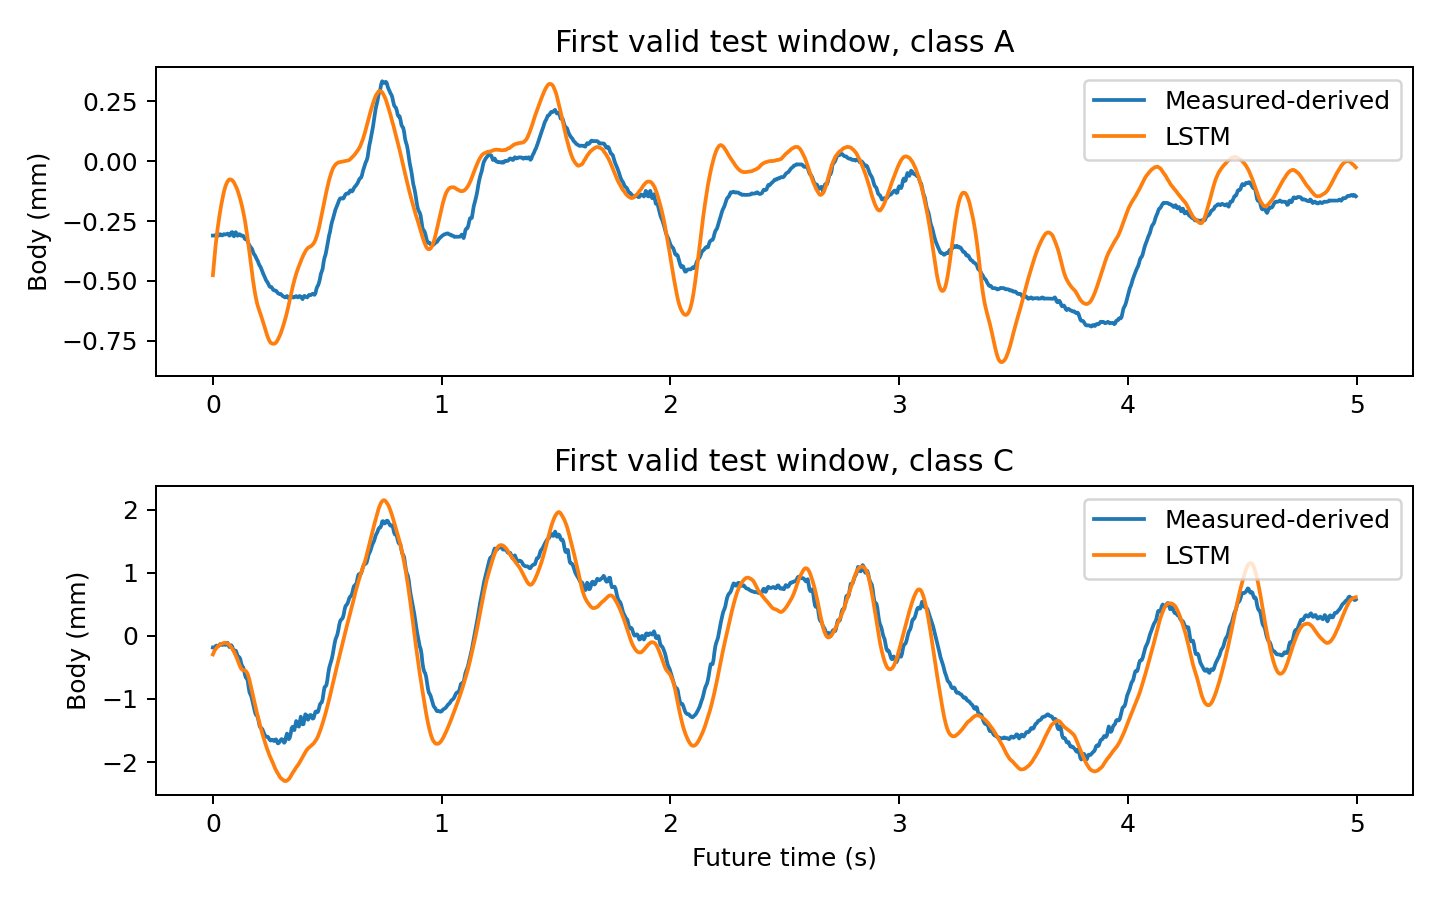
\includegraphics[width=\columnwidth]{../figures/forecast.png}
\caption{Primeira janela válida do teste em A e C, modelo global, semente 42. A seleção segue a ordem temporal, não o menor erro. Os deslocamentos medidos são processados.}
\label{fig:forecast}
\end{figure}

A Fig.~\ref{fig:forecast} ilustra tendências acompanhadas e variações não reproduzidas. Calcular conforto diretamente da aceleração temporal da LSTM global produziu acurácia entre 45,6\% e 57,8\%, inferior à cabeça agregada. Logo, boa classificação não valida toda a trajetória de aceleração nem a consistência física entre as saídas.

Em C, sempre indicar desconforto permite 100\% de acerto, sem demonstrar discriminação binária. A LSTM especializada obteve RMSE de 0,254 mm, ante 0,289 mm do global nesse mesmo teste C. A diversidade não melhorou automaticamente essa classe, e a diferença na quantidade de treino impede isolar seu efeito.

A separação dos rótulos por classe sugere um fator de confusão: reconhecer amplitudes associadas à rugosidade pode explicar parte do desempenho, sem aprender transições de conforto dentro de cada classe. A ausência de falsos confortos nesse teste correlacionado não deve ser generalizada. Na demonstração salva, 0,6 Hz de frequência prevista coexistiu com RMS aprendido próximo de 0,750 m/s$^2$, ilustrando que até 2 Hz não substitui um indicador de intensidade.

As principais limitações são a sensibilidade da aceleração derivada ao filtro e ao ruído, a quantidade limitada de realizações, a correlação entre repetições, a hipótese de pista futura conhecida e a ausência de assento e passageiros. Não se variaram parâmetros mecânicos da suspensão. A classificação é concordância com um alvo numérico de bancada.

\balance
\section{Conclusão}
Implementou-se um fluxo reproduzível de previsão condicionada, treinamento por uma ou cinco classes e decisão aproximada de conforto. A cabeça agregada LSTM melhorou a classificação global frente às referências avaliadas; o ARX apresentou menor erro temporal. Os achados justificam separar qualidade da trajetória e do indicador.

Trabalhos futuros devem validar aceleração com sensores independentes, coletar novas realizações e ambos os rótulos dentro de cada classe, além de avaliar assento e passageiros antes de extrapolar conforto. Código, pesos e métricas estão em \url{https://github.com/pedruck/ia-ii-suspensao}.

\begin{thebibliography}{4}
\bibitem{dataset} M. Foo and A. H. Tan, ``Benchmark vehicle suspension data based on ISO 8608 road profiles,'' Zenodo, v3, 2025, doi: 10.5281/zenodo.17242919.
\bibitem{benchmark} M. Foo and A. H. Tan, ``Benchmark vehicle suspension data based on ISO 8608 road profiles,'' \emph{Control Engineering Practice}, vol. 169, art. 106755, 2026, doi: 10.1016/j.conengprac.2025.106755.
\bibitem{vasquez} F. A. Vasquez Stuardo, \emph{Optimisation of off-road motorcycle suspensions}, doctoral thesis, University of Southampton, 2020, Appendix A.4. [Online]. Available: \url{https://eprints.soton.ac.uk/448147/}
\bibitem{comfort} R. Wawryszczuk, E. Kardas-Cinal, J. Lejk and M. Sokolowski, ``Methods of Passenger Ride Comfort Evaluation---Tests for Metro Cars,'' \emph{Sensors}, vol. 23, no. 12, art. 5741, 2023, doi: 10.3390/s23125741.
\end{thebibliography}
\end{document}
